\chapter{Introduction}
\label{chap:intro}

\section{The Monte Carlo Method}

At the heart of nuclear engineering and many associated fields is the study of
the behavior of subatomic particles interacting with matter. Reactor engineers
are interested in the distribution of power and other reaction rates at each
point in a nuclear reactor; medical physicists are interested in energy
deposition in the human body due to radiation treatments; nuclear
astrophysicists are interested in how nuclear reactions can produce elements
heavier than hydrogen in stars; and so on. In order to determine such
quantities, one generally needs knowledge of two things:
\begin{enumerate}
\item An understanding of how individual particles interact with the matter
  through which they're traveling; and
\item A mathematical description for how a distribution of particles evolves in
  time.
\end{enumerate}
The study of particle interactions is of primary concern to nuclear
physicists. The advent of quantum mechanics in the early 20th century greatly
advanced the state of understanding of particle interactions, especially with
respect to the scattering of particles, a subject which can not be understood
well without considering quantum effects. The latter subject, i.e. the theory of
particle transport, came to maturity in the middle and later parts of the 20th
century, with many advances coming from the nuclear reactor engineering
community which was focused on studying the behavior of fissionable systems.

The physical transport of particles is stochastic and non-deterministic; a free
particle moving through a medium, after being born from some nuclear, chemical,
or other process, will have a trajectory consisting of a number of successive
random steps (a random walk). At the end of this random walk, the particle is
absorbed, transmuted, or otherwise ``killed''.  To cast the problem into a
strictly mathematical form, it is necessary to make a continuum hypothesis. This
hypothesis implies that the particle density is high enough such that over the
length scales (be it in space, energy, or time) one is interested in, the
average behavior of particles will be observed. In certain situations, e.g. a
reactor operating at very low power, the continuum hypothesis may not be valid,
and the actual behavior of particles at any given point in phase space may
deviate significantly from its average. However, for most practical cases of
interest in nuclear engineering, the particle densities are indeed high enough
to justify the continuum hypothesis. The equation that results from this
hypothesis is known as the Boltzmann transport equation.

There are two fundamentally different approaches for determining the
distribution of particles in a system:
\begin{enumerate}
\item \emph{Monte Carlo methods} model particle transport\footnote{It is to be
  understood that while the term \emph{Monte Carlo} applies to a very wide class
  of statistical simulation techniques, we will be focusing solely on Monte
  Carlo methods as applied to particle transport.} by mimicking the actual
  physical transport of particles using fictitious ``particles'' --- variables
  stored in computer memory representative of a position, direction, and
  energy. At each stage in an actual particle's life, there is a known
  probability distribution for the distance it travels between collisions, the
  probability of undergoing a certain reaction, and the energy and angle
  following a collision/reaction. By successively sampling these known
  probability distributions, the life of a particle can be simulated from birth
  to death. This process is repeated until enough particles have been simulated
  to obtain the average behavior with sufficiently low statistical uncertainty.
\item \emph{Deterministic methods} determine the average behavior of particles
  in a system by numerically solving the Boltzmann transport equation. This
  requires discretizations of each of the phase space variables: space, angle,
  and energy.
\end{enumerate}
While these two approaches can be shown to be equivalent to one another, there
are various trade-offs and incentives for using one method or the other. It
should also be noted that deterministic methods encompass a wide variety of
solution and discretization techniques, e.g. discrete ordinates
\cite{carlson-1965}, spherical harmonics \cite{bell-1970}, and the method of
characteristics \cite{physor-smith-2002}.

In this thesis, we will focus specifically on the transport of neutrons through
a multiplying (fissionable) medium --- a topic that is central to the study of
energy production in nuclear reactors. When a fissionable medium is present, a
source of neutrons is introduced that is itself proportional to the neutron
population. As a result, the steady-state neutron transport equation is
generally solved as an eigenvalue equation where the eigenvalue represents a
scaling factor on the fission source that forces the equation to balance. More
specifically, the solution of the neutron transport equation via Monte Carlo
methods will be studied in the context of massively parallel simulations on
supercomputers. Neutron transport has a few desirable characteristics. Neutrons,
being neutral particles, are generally not subject to external forces when
traveling between collisions. Moreover, it is not necessary to consider
collisions between neutrons since the density of the host medium is generally
much greater than the density of neutrons\footnote{Another way of thinking about
  this is that the particles and the host medium can be considered mutually
  exclusive.}. This property enables the simulation of neutrons via Monte Carlo
methods to be parallelized quite easily since the trajectory of each particle is
completely independent of all others.

\section{History of Parallel Algorithms}

The ability to simulate complex transport phenomena using stochastic methods was
recognized early on in the development of multiplying fission systems. Also
recognized was the fact that while providing an elegant means of computing
functionals, such methods would require a great amount of computation as
well. The development of Monte Carlo methods has thus gone hand-in-hand with the
development of computers over the course of the last half century.

Due to the computationally-intensive nature of Monte Carlo methods, there has
been an ever-present interest in parallelizing such simulations. Even in the
first paper on the Monte Carlo method \cite{jama-metropolis-1949}, John
Metropolis and Stanislaw Ulam recognized that solving the Boltzmann equation
with the Monte Carlo method could be done in parallel very easily whereas the
deterministic counterparts for solving the Boltzmann equation did not offer such
a natural means of parallelism. With the introduction of vector computers in the
early 1970s, general-purpose parallel computing became a reality. In 1972,
Troubetzkoy et al. designed a Monte Carlo code to be run on the first vector
computer, the ILLIAC-IV \cite{trans-troubetzkoy-1973}. The general principles
from that work were later refined and extended greatly through the work of
Forrest Brown in the 1980s \cite{pne-brown-1984}. However, as Brown's work
shows, the single-instruction multiple-data (SIMD) parallel model inherent to
vector processing does not lend itself to the parallelism on particles in Monte
Carlo simulations. Troubetzkoy et al. recognized this, remarking that ``the
order and the nature of these physical events have little, if any, correlation
from history to history,'' and thus following independent particle histories
simultaneously using a SIMD model is difficult.

The difficulties with vector processing of Monte Carlo codes led to the adoption
of the single program, multiple data (SPMD) technique for parallelization, first
proposed in general form in 1984 at IBM \cite{pvmmpi-darema-2001}. In this
model, multiple processors simultaneously execute a program independently of one
another. As applied to Monte Carlo particle transport, this means that each
different process tracks a particle independently of other processes. However,
it is still necessary to exchange some data between processes. For example,
tally results from each process need to be added together to obtain a final
result. This and other data can be exchanged between processes through a
\emph{message-passing} interface.

The SPMD technique became widespread once message-passing standards were
introduced in the late 1980s and early 1990s such as PVM
\cite{ornl-beguelin-1991} and MPI \cite{gropp-1999}. Over time, the SPMD model
has proved much easier to use than vectorization methods in practice and takes
advantage of the inherent parallelism on particles rather than instruction-level
parallelism. As a result, it has since become ubiquitous for Monte Carlo
simulations of transport phenomena. The SPMD parallel model has enabled high
parallel efficiencies in Monte Carlo codes using small clusters.

\section{Motivation}

At the present time, Monte Carlo neutron transport simulations are primarily
used for benchmarking and validation purposes. In some cases, research or test
reactors can also reasonably be simulated directly using Monte Carlo
\cite{anfm-romano-2009}. For these types of applications, simulation on a small
cluster (via SPMD parallelism) is usually sufficient to obtain a solution with
acceptably low statical uncertainties within a short amount of time. However,
the use of Monte Carlo methods to directly simulate large commercial nuclear
reactors has been viewed as impractical due to the excessive computational
burden. Instead, reactor core analysis codes have traditionally been based on
deterministic methods. Furthermore, at the level of full-core simulation, nodal
diffusion methods are typically employed.

The use of diffusion theory introduces approximations that are sometimes not
very accurate, particularly with respect to leakage and the presence of strong
absorbers. To overcome these approximations, one solution is to simply avoid the
diffusion approximation and use deterministic transport methods such as discrete
ordinates or method of characteristics. However, these methods are, in practice,
quite difficult to use at the level of full-core simulation. Again, these
methods rely on discretization --- this means that the discretized mesh over
which the problem must be solved will grow in proportion to the physical size of
the problem. Ergo, the solution time and memory requirements will also grow with
increases in the physical size of the problem. Seen this way, accurate solution
of full-core reactor problems using transport theory, regardless of whether it
is by Monte Carlo or deterministic methods, will require large-scale
high-performance computing (HPC) resources coupled with parallel algorithms that
will scale to thousands or possibly millions of processors.

Monte Carlo methods offer several potential advantages over deterministic
methods, particularly in areas that tend to encumber the practical adoption of
transport tools to new classes of problems: the avoidance of complex meshing for
complicated geometries, the simplification of the cumbersome multi-group cross
section generation process, and, perhaps most importantly, the potentially
easier adaptability to the extreme levels of concurrency that are likely to
characterize beyond-petascale HPC architectures. Notwithstanding these
advantages, there are a number of algorithmic shortcomings that would prevent
the immediate adoption of Monte Carlo methods for full-core analyses. Before
discussing explicitly the algorithmic shortcomings related to full-core reactor
simulation using Monte Carlo and potential solutions, it helps first to set the
stage by introducing contemporary ``challenge problems''. With these problems as
a reference point, the limitations of present parallel methods should then
become evident.

\section{Challenge Problems}

\subsection{NEA Monte Carlo Performance Benchmark}

In 2003, Kord Smith issued a challenge by predicting that the solution to a
full-core reactor problem using Monte Carlo methods would not be possible on a
single CPU in under an hour until the year 2030 \cite{mc-smith-2003}. In his
lecture, Smith specified that the local power in each pin subdivided into 100
axial and 10 radial zones be calculated to within 1\% statistical uncertainty.
Smith's 2030 estimate was later refined by Martin in an invited talk at the M\&C
2007 conference \cite{mc-martin-2007}, who estimated that it would take until
year 2019. Hoogenboom and Martin then proposed a full-core benchmark problem
\cite{mc-hoogenboom-2009} at the M\&C 2009 conference called the Monte Carlo
performance benchmark that would serve as a reference for monitoring progress
towards reaching the Kord Smith challenge. The benchmark model consists of a
pressurized water reactor with 241 assemblies, each containing a 17 by 17 square
rod array. The original version of the benchmark also included five fuel pins
with Gadolinium within each assembly as well as two different assembly types
having asymmetric positions. However, a later specification of the benchmark
\cite{mc-hoogenboom-2011} removed the five Gadolinium pins in each assembly
(instead, every pin has Gd) and the asymmetries by having only one assembly
type. The later specification also included 25 control rod guide tubes in each
assembly. \autoref{fig:mcperformance} shows the general geometric layout of the
revised benchmark.
\begin{figure}
  \centering
  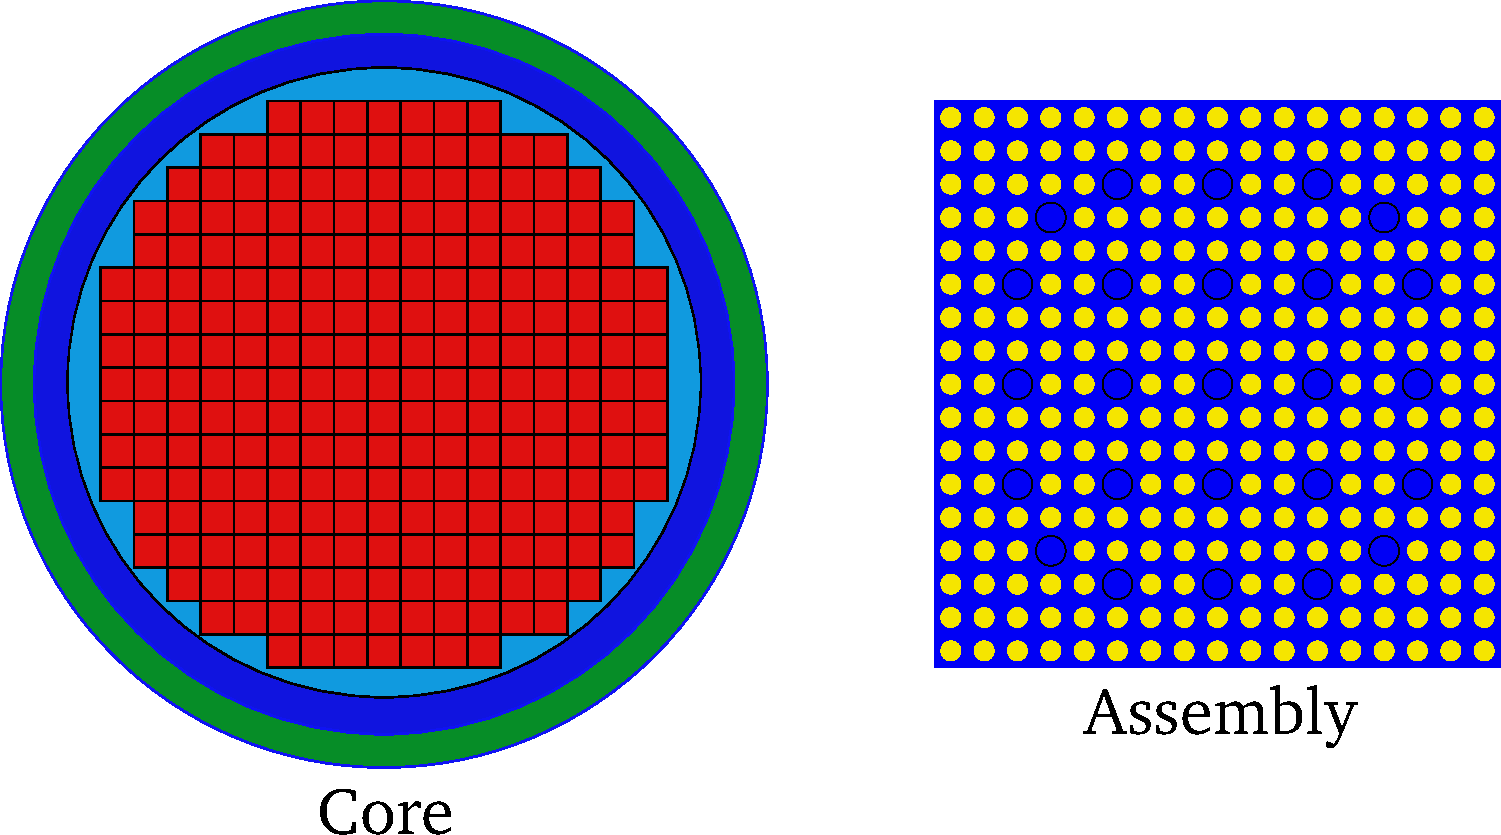
\includegraphics[width=5.0in]{figures/ch1/mcperformance.pdf}
  \caption{Geometry layout of the NEA Monte Carlo performance benchmark.}
  \label{fig:mcperformance}
\end{figure}

There are a number of simplifications in the Monte Carlo performance benchmark
model that make it quite unrealistic as far as light-water reactor (LWR) design
is concerned. There are no control rods, no core baffle, no grid spacers, and
very limited ex-core detail. Furthermore, the fact that all fuel pins are the
same enrichment and composition results in a roughly cosine distribution in the
axial direction and a Bessel distribution in the radial direction. All materials
in the problem are also specified to use cross sections at a single
temperature. Nevertheless, even this simplified problem is computationally
challenging due to the number of unknowns to be solved for. In this benchmark,
the aim is to compute the power distribution for every fuel pin subdivided into
100 evenly spaced axial nodes (note that the 10 radial rings per pin originally
specified by Smith were not included). With 264 fuel pins in each assembly and
241 assemblies, this means there are 6,362,400 unique regions that need to be
tallied over.

At the PHYSOR 2010 conference, Kelly et al. presented the first credible
solution to the Monte Carlo Performance benchmark \cite{physor-kelly-2010} using
the MC21 Monte Carlo code \cite{mc-sutton-2007} developed by the Knolls and
Bettis Atomic Power Laboratories. To solve for the local power distribution, a
simulation was run with 40 billion active neutron histories and the flux, total
absorption rate, and total fission rate were tallied over a pin cell mesh with
100 axial mesh cells. They faced a number of challenges and problems in their
solution:
\begin{itemize}
\item Even with 40 billion neutrons, virtually none of the local tallies had
  95\% confidence intervals with half-widths of less than 1\% of the mean as
  required by the Kord Smith Challenge.
\item Due to the highly non-uniform nature of the power distribution, regions of
  the problem with low fission rate density had correspondingly large variances.
\item Although the tallies in their simulation required about 0.5 GB of memory,
  the problem overall took over 6 GB. Since the SPMD method implies that all
  memory is replicated across different processes, the memory requirements could
  easily exceed that available on a single node. In their case, they had at
  least 24 GB of memory shared among four cores.
\item Since the benchmark model has a dominance ratio close to unity, Kelly et
  al. had to use 300 inactive batches before tallies even began to accumulate.
\end{itemize}
Their simulation ran for 18 hours on 400 processors, implying that on a single
processor it would have taken about 300 days.

Leppänen analyzed the Monte Carlo performance benchmark using the Serpent Monte
Carlo code \cite{vtt-leppanen-2007} and presented results at the SNA + MC2010
conference \cite{sna-leppanen-2010}. In his simulation, 100 billion active
neutron histories were used. Thanks to use of delta tracking and various methods
that enable a faster simulation at the expense of more memory in Serpent, the
simulation took about 21 days on 7 processor cores, a rate twice as fast as that
obtained in Kelly et al.'s 2010 analysis. No mention was made of the exact
memory requirements for the simulation.

At the PHYSOR 2012 conference, Kelly et al. gave an updated solution to the
Monte Carlo performance benchmark, again using MC21 but incorporating a few new
methods \cite{physor-kelly-2012}. The first modification was that they used
multiple fission generations per batch to eliminate the systematic
underprediction of confidence intervals. In addition, they introduced a new
methodology for weighting the fission source sites at each batch to achieve a
flatter variance distribution. With these two methods, they ran a simulation
with 200 billion active neutron histories and succeeded in reaching the
criterion of having 95\% of tallies with 95\% confidence intervals with half
widths of less than 1\% of their respective means. This simulation took 75.6
hours on 750 processor cores.

\subsection{MIT PWR Benchmark}

The introduction of the NEA Monte Carlo performance benchmark was an important
first step in encouraging the Monte Carlo community to start addressing problems
related to the ability to perform full-core simulations. The analyses by Kelly
et al. and Leppänen have shown that obtaining a solution is indeed possible
given the availability of large computing resources. However, as previously
mentioned, the benchmark model contains many model simplifications that make the
problem unrealistic.

To move towards simulation of actual reactor models, MIT is currently developing
a PWR full-core benchmark that includes details and dimensions from an actual
operating PWR plant. Many of the simplifications that were present in the NEA
Monte Carlo performance benchmark are not part of the MIT benchmark; features
that are explicitly modeled include radial enrichment zoning, guide tubes and
instrument tubes, burnable absorbers and control rods, grid spacers, core
support, core baffle, core barrel, thermal shield pads, and the reactor pressure
vessel. A geometry plot of the benchmark model is shown in
\autoref{fig:mit-pwr-benchmark}.
\begin{figure}[htb]
  \centering
  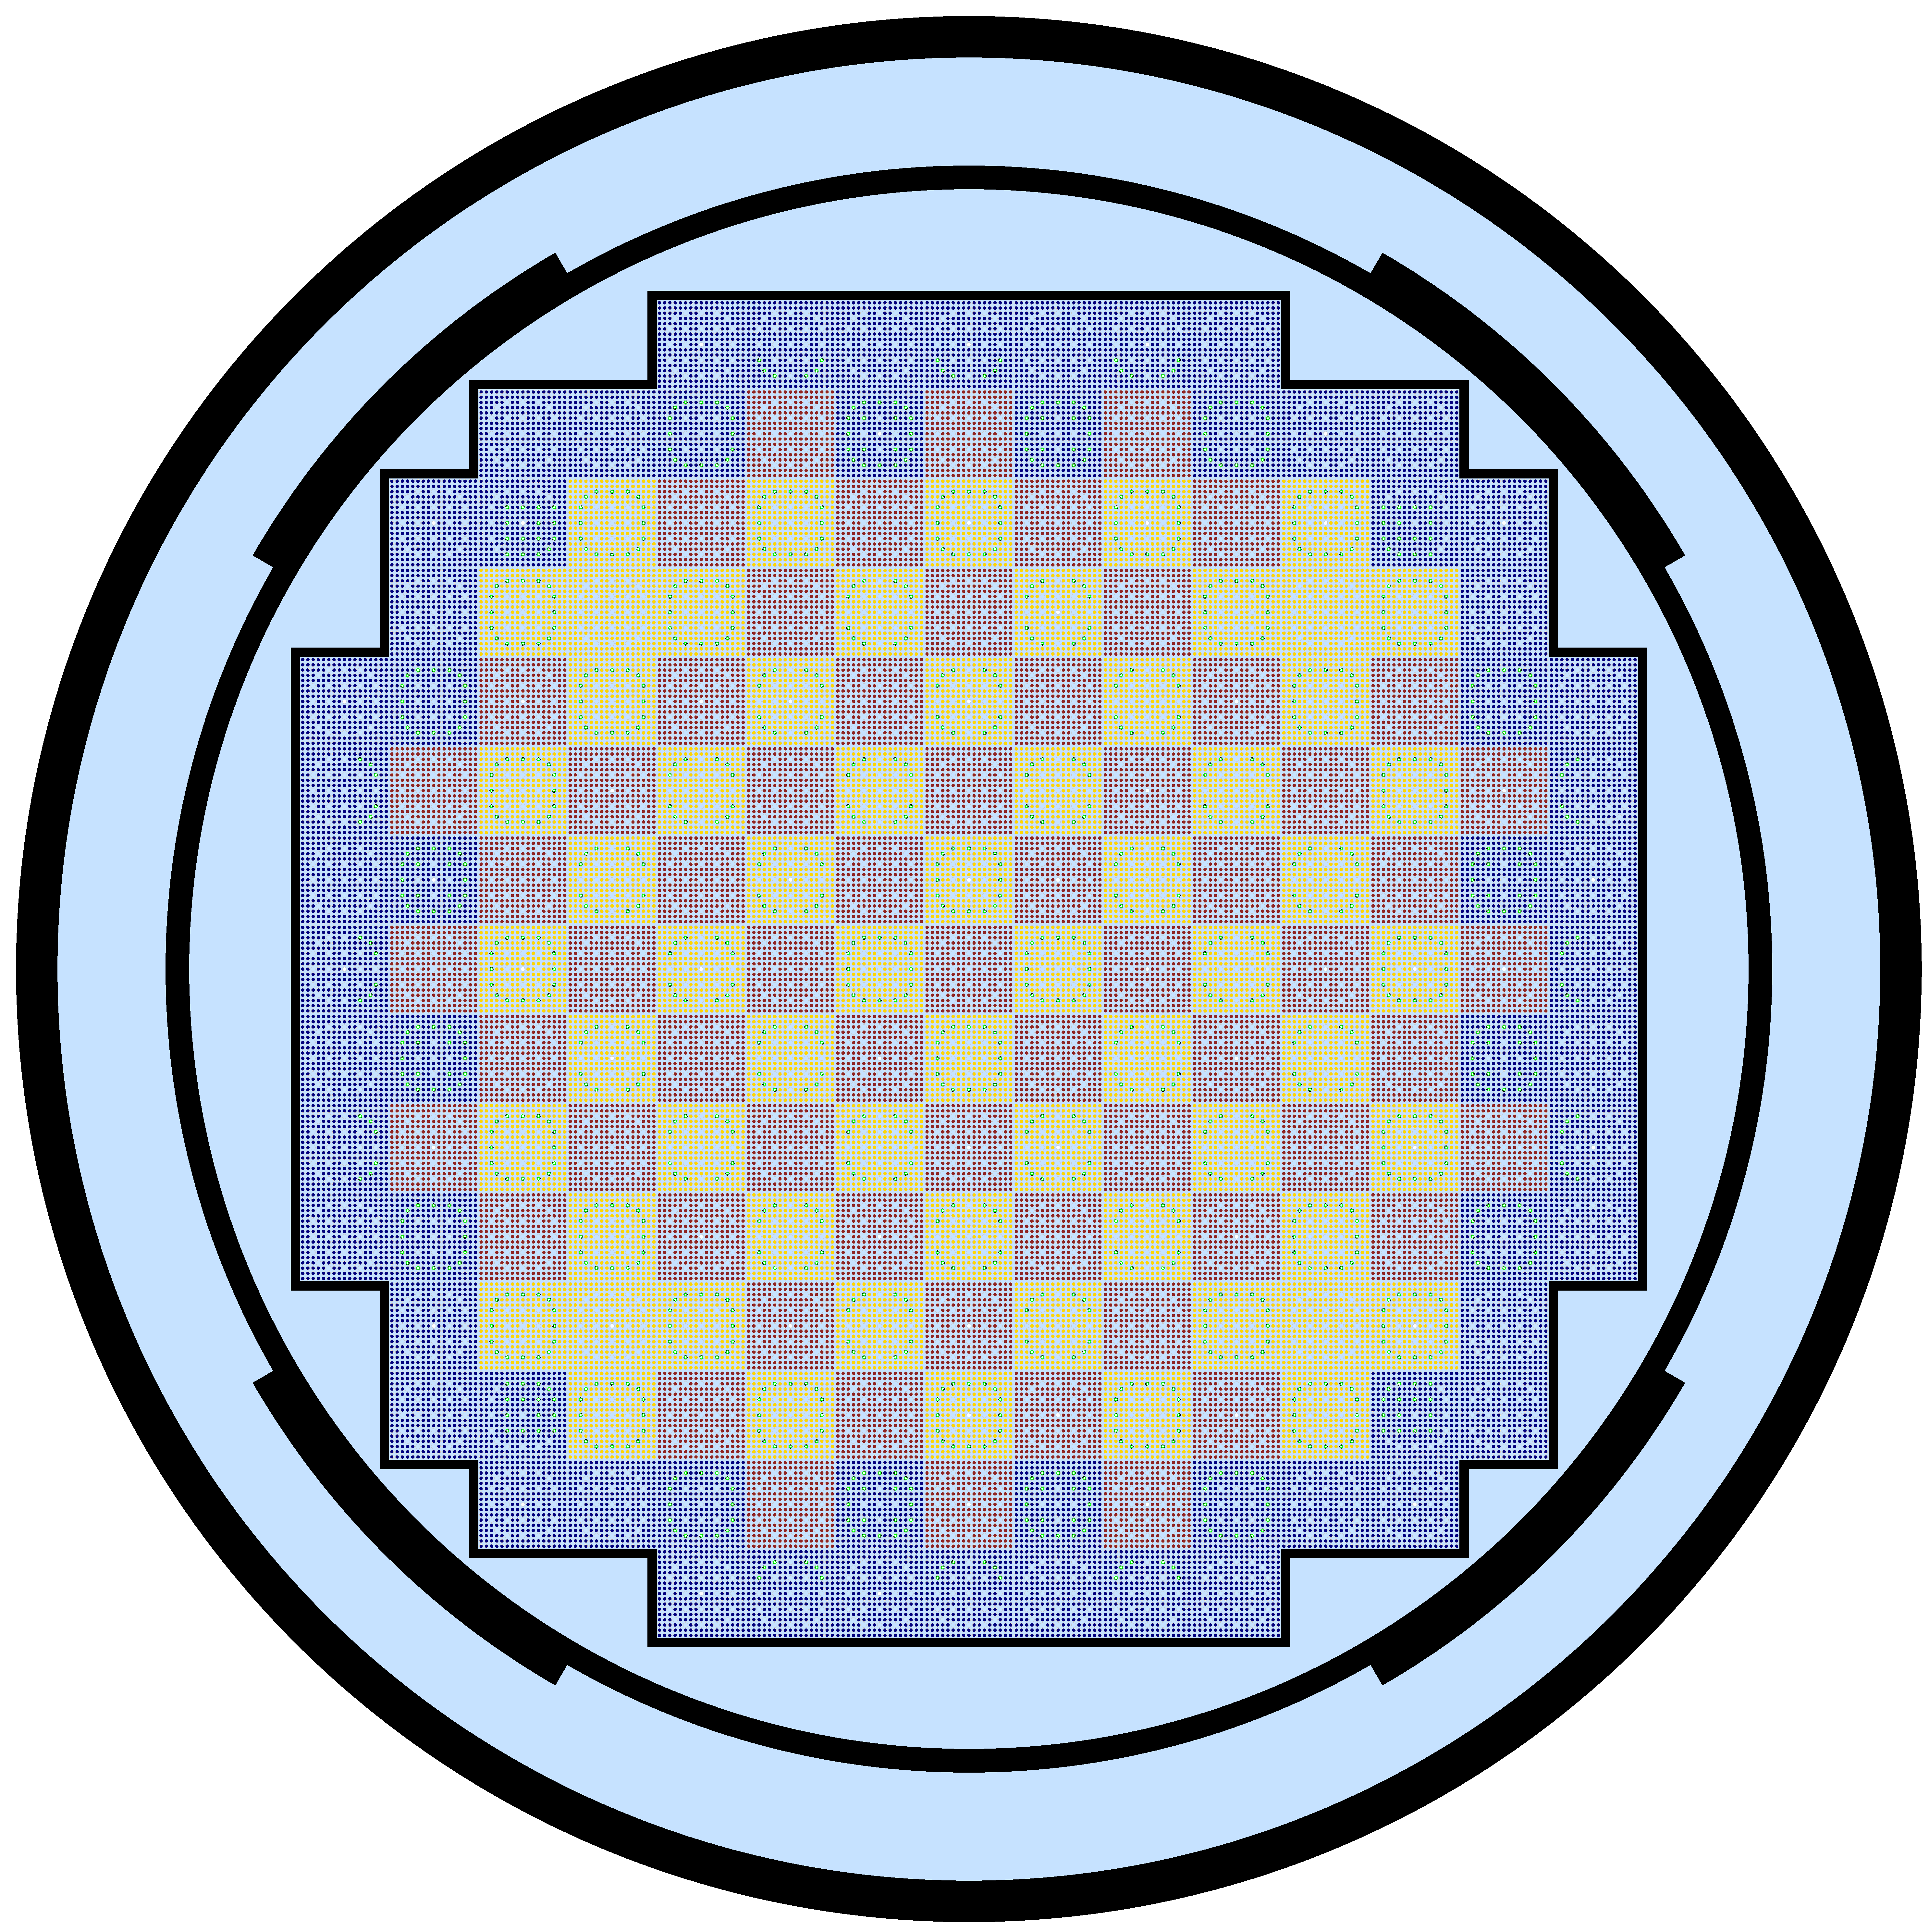
\includegraphics[width=4.0in]{figures/ch1/mit-pwr-benchmark.png}
  \caption{Geometry plot of a preliminary model of the MIT PWR Benchmark
    generated with the OpenMC Monte Carlo code.}
  \label{fig:mit-pwr-benchmark}
\end{figure}
The level of detail and complexity in the MIT benchmark will only exacerbate the
challenges encountered when simulating the Monte Carlo performance benchmark
including high memory requirements, poor source convergence, and the requirement
to run possibly trillions of particles to reach convergence of local tallies.

\section{Summary of Issues}

As we see from the preceding considerations, there are a number of formidable
challenges to simulating full-core reactor problems directly using Monte
Carlo. Perhaps the most important point to recognize (as it indirectly or
directly causes all other problems), is that to obtained a converged solution
for the spatial distribution of power in a full-core model will likely require
an unprecedented number of particle histories. The study of Kelly et
al. \cite{physor-kelly-2012} showed that even for the simplified NEA Monte Carlo
performance benchmark, 200 billion active neutron histories were required to
converge the local tallies. To accurately model changes in material compositions
due to depletion, it is likely that as many as 500 axial nodes will be required
instead of 100; on top of that, 10 radial rings per pin may be necessary. Thus,
assuming the number of particles needed to reach the desired uncertainty
criterion scales with the number of tally regions, we would need $200 \cdot 10^9
\times 5 \times 10 = 10 \cdot 10^{12}$, or ten trillion, neutrons to fully
converge all tallies.

Barring a huge increase in the efficiency of single processor cores, the
expedient solution of a full-core reactor problem will in turn require millions
of processors running simultaneously. To-date, only a few studies in the
literature have demonstrated the use of even thousands of processors in parallel
in a Monte Carlo neutron transport simulation \cite{lanl-brown-2005,
  ane-romano-2013}.

Let us now discuss each algorithmic issue in further detail to assess 1) whether
solutions to these problems already exist, 2) the status of current work towards
their resolution, and 3) what areas need further work. It is the last point that
motivates the objective of this thesis. 

\subsection{Source Convergence}

In a Monte Carlo $k$-eigenvalue calculation, we start with some assumed guess of
the actual fission source distribution. Before tallies can begin accumulating,
it is necessary to first iterate on the fission source to obtain a converged
distribution. The rate at which the fission source distribution will converge
depends on a quantity known as the \emph{dominance ratio}, the ratio of the
first higher harmonic eigenvalue to the fundamental mode eigenvalue. The closer
the dominance ratio is to one, the more difficult it is to converge the fission
source distribution.

In a typical commercial light-water reactor, the width and height of the reactor
core are very large relative to the mean free path of neutrons. As a result,
full-core reactor models typically have dominance ratios close to
unity. Converging on the fission source distribution can consequently require
hundreds of iterations if using standard power iteration. With a small batch
size, this might not be much of a concern. However, in a simulation with
possibly millions of processor cores, each one must be occupied with sufficient
work. As a result, batch sizes with many billions of particles would be needed
in practice. If we are to discard hundreds of batches, each composed of billions
of particles, at the beginning of every simulation, a great amount of processor
time may be wasted.

A number of solutions have been proposed to obtain faster fission source
convergence in Monte Carlo $k$-eigenvalue calculations. These include the
fission matrix method \cite{ane-dufek-2007, lanl-carney-2012}, Wielandt's method
\cite{jnst-yamamoto-2004, mc-brown-2007}, extrapolation methods
\cite{mc-toth-2007-1, mc-toth-2007-2}, and acceleration via low-order operators
(e.g. coarse mesh finite difference \cite{physor-lee-2010, sna-lee-2010,
  physor-lee-2012}), to name a few. Lee et al. \cite{physor-lee-2012} have
demonstrated that the CMFD formulation can reduce the number of inactive batches
in an eigenvalue calculation to less than 20 with effectively no overhead from
solving the low-order CMFD system. With this and other viable solutions at hand,
source convergence is now considered by many in the Monte Carlo community to be
a solved problem. Methods to accelerate fission source convergence have been or
are currently being implemented in a number of Monte Carlo codes including MCNP
\cite{lanl-young-2011}, MC21, and OpenMC \cite{mc-romano-2013}.

While source convergence may now be of less concern than it was years ago thanks
to effective acceleration methods, the diagnosis and suppression of tally bias
due to undersampling \cite{nse-ueki-2005, nse-ueki-2008, jnst-ueki-2011} is
still an outstanding problem. However, this is primarily a physics problem that
will not impede the successful implementation of scalable parallel
algorithms. As such, it is not explored in this thesis.

\subsection{Cross Section Memory Requirements}
\label{sec:cross-section-memory}

One of the simplifications in the NEA Monte Carlo performance benchmark is that
all materials are to be treated at the same temperature. This was done for
practical purposes as it allows someone simulating the benchmark to use cross
section data processed at a single temperature (in this case room
temperature). However, for problems containing nuclides at many temperatures
(e.g. a reactor at full power), or with time-varying temperatures, it is
necessary to store cross sections at many temperatures.

The next natural question is then --- how many temperatures are necessary? This
question was studied in some depth by Trumbull \cite{nt-trumbull-2006}. He
concluded that for many nuclides, cross sections would need to be stored at
increments of less than 28 K. Assuming that even a 28 K interval were
sufficient, this means that over the range of temperatures found in a
light-water reactor (typically 293 K up to at least 1300 K for steady state
calculations and 2500 K for transients), cross sections would be needed at over
75 different temperatures. Thus, potentially hundreds of GB of memory are needed
to accommodate cross sections for a truly temperature-dependent model. The
reader should once again recall that, in the standard SPMD parallel model, this
memory requirement is to be multiplied by the number of processes used in the
simulation. It is thus anticipated that special techniques will need to be
employed in order to perform massively-parallel full-core LWR simulations given
that the memory requirements will almost certainly exceed the available node
memory.

Two solutions for reducing cross section memory requirements have thus far been
proposed. The first method is known as on-the-fly Doppler broadening
\cite{nse-yesilyurt-2012, trans-brown-2012}. The basic idea is that the cross
section at any temperature can be represented as a series expansion. As a
result, only the 0 K cross sections and a series of expansion coefficients need
be stored in memory. While this method does show some promise, it may not
ultimately be an adequate solution for LWR simulation since the range of
temperatures and required accuracy could necessitate that the series expansion
contain at least 13 terms and possibly more for certain nuclides
\cite{net-martin-2012}. Thus, the problem is merely shifted from storing cross
sections at a multitude of temperatures to storing a multitude of series
expansion coefficients.

Another method that may potentially solve the cross section memory requirements
is the work of Viitanen on explicit temperature treatment
\cite{nse-viitanen-2012, physor-viitanen-2012}. This method would enable
simulation using 0 K cross sections via a rejection technique based on Woodcock
delta tracking. The downside is that the method may incur a performance
penalty. However, from the perspective of massively parallel simulations, the
trade-off of a slower calculational rate in return for drastically reduced
memory requirement is quite tolerable. It is often said that ``flops are free''
\cite{sc-panel-2009}; on the other hand, memory is an increasingly scarce
resource for high fidelity simulations. Given that excellent progress has been
made towards reducing cross section memory requirements, it is a topic that will
not be further explored as part of the current work.

\subsection{Tally Memory Requirements}
\label{sec:tally-memory}

Kelly et al. \cite{physor-kelly-2012} found that the memory required in their
simulation of the Monte Carlo performance benchmark was so large that they were
unable to use all processors on a single node. For that problem, the tallies
consumed about 0.5 GB on each process --- a number that actually may not, at
first glance, seem that prohibitive. However, we must keep in mind the following
facts: 1) they were only solving for a few (three) physical quantities for each
tally region, and 2) the number of regions they used may be 50 times smaller
than that needed for a realistic reactor simulation.

If we were really only interested in a steady-state problem, it would suffice to
calculate just the total energy deposition in each tally region and perhaps a
few more quantities. However, the fuel composition will slowly change over time
due to irradiation and depletion of the fuel. Furthermore, while fresh fuel in a
reactor may be composed of only a few nuclides, over time hundreds of actinides
and fission product nuclides will appear in the fuel due to nuclear
transmutation. This process is governed by a set of equations called the Bateman
equations \cite{ane-cetnar-2006}. In order to solve the Bateman equations, one
needs to know various reaction rates in each nuclide in the fuel: the fission
reaction rate, the $(n,\gamma)$ reaction rate, the $(n,2n)$ reaction rate, the
$(n,3n)$ reaction rate, the $(n,\alpha)$ reaction rate, and the $(n,p)$ reaction
rate.

To get an idea for just how large the memory requirements for tallies might be,
let us consider a depletion simulation of the MIT PWR benchmark. This benchmark
has 193 assemblies, each having 264 pins. With 500 axial and 10 radial zones
within each fuel pin for depletion purposes, the total number of depletable
materials would be 254,760,000. With approximately 300 nuclides and six reaction
rates needed for each nuclide, the total memory for tallies would be
$254,760,000 \times 300 \times 6 \times 24$ bytes\footnote{We have chosen the
  last multiplier as 24 bytes for the following reason; for each tally bin we
  need to store the accumulated sum, the accumulated sum of squares, and also a
  temporary variable that is used for a single batch. Thus there are three
  8-byte floating point numbers.} = 11,005,632,000,000 bytes or \textbf{11
  terabytes}. Again, in the SPMD parallel model, this amount of memory would be
required for each process. This is clearly a major problem and one that has no
easy resolution.

One of the primary objectives of this thesis is to study algorithms for
decomposing tally memory and provide guidance on the best path going forward for
realistic LWR analysis. Two classes of strategies have been proposed to address
this problem --- what we loosely refer to as \emph{data decomposition} and
\emph{domain decomposition}. Data decomposition could take many forms, but the
basic approach would involve the same naturally parallel by-particle
parallelization strategy as is currently employed together with a set of
dedicated \emph{tally servers} that continuously receive tally updates from the
tracking processors (e.g. with one-side operations or by running a continuous
receive loop). The spatial decomposition of the tallies is in general arbitrary
and the data sent from the tracking processors could be carried out with
non-blocking MPI send operations to maximize overlap in
communication/computation.

Domain decomposition on the other hand associates a contiguous region of
physical space with each processing element (or node). Each processor then owns
the subset of tallies for the corresponding region of physical space. This
approach is potentially made efficient with a more complex parallelization
strategy where each processor only tracks the particles that are passing through
its own portion of the domain.  However, new complexities emerge --- fast
neutrons travel long distances before absorption, and thus the local leakage
rates (probability of a neutron leaving a partition before being absorbed) are
relatively large. This requires intermediate data exchange \emph{stages} where
particles are moved to adjacent processors, potentially leading to significant
communication costs and non-trivial load imbalances.

\subsection{Degradation of Parallel Efficiency}

Thus far, we have discussed algorithmic problems that arise when simulating
full-core reactor models, regardless of how many processors are utilized. The
full-core LWR simulations that have been performed to date
\cite{sna-leppanen-2010, physor-kelly-2012} have generally used under 1000
processors. With this many processors, overhead from network communication is
generally small compared to the overall computation time, especially when using
a high-speed network interconnect. However, more realistic reactor simulations
will require trillions of particles and hence orders of magnitude greater
processor core counts. That being the case, the network communication from
message-passing can quickly become prohibitive if scalable algorithms are not
utilized. Until recently, Monte Carlo particle transport simulations using this
many processors had not been attempted --- in fact, the first attempts at such
large runs are presented in this thesis.

It has been fairly well-documented that current production Monte Carlo codes,
such as MCNP \cite{nt-goorley-2012}, do not scale well to large numbers of
processors. So bad is the problem that a prominent researcher has recently
questioned whether Monte Carlo truly ``is ... embarrassingly parallel''
\cite{physor-hoogenboom-2012}. The inability to achieve scaling can be traced to
one fundamental design flaw. Most parallel algorithms in Monte Carlo codes are
commonly implemented in the form of a \emph{master-slave} algorithms. This means
that one process acts as the \emph{master}, assigning and coordinating work
between all other \emph{slave} processes. While master-slave algorithms can be
beneficial from the perspective of maintaining good load balancing, they can
also unfortunately create a bottleneck at the master process. In practice, poor
scaling can result from two distinct algorithms:
\begin{enumerate}
\item \emph{Fission source synchronization} --- in an eigenvalue calculation, it
  is necessary to iterate over the fission source to obtain a converged
  distribution. During each fission source iteration, source sites are generated
  as fission occurs and are stored in an array called the \emph{fission
    bank}. As the generation of these sites is stochastic, we may end up with
  fewer or more sites than particles requested per source iteration. Thus the
  specified number of sites must be sampled from the fission bank. Common
  implementations rely on a single master processor to
  sort/re-order\footnote{This is done for the sake of maintaining
    reproducibility, which is discussed at length in
    \autoref{chap:fission-bank}.}, sample, and redistribute all source sites.
\item \emph{Tally reduction} --- in many Monte Carlo codes, each process
  responsible for tracking particles accumulates its own estimates of the tally
  random variables. At the end of every realization, these estimates are added
  together to obtain a single estimate (with lower variance). In terms of
  network communication, this requires that the tallies be \emph{reduced} from
  all processors to one, a process which can take $O(p \log_2 p)$ steps where
  $p$ is the number of processes. This generally affects both fixed source and
  eigenvalue calculations, but is only a problem when many tally bins are
  used. We saw earlier that for realistic reactor calculations, terabytes of
  memory corresponding to many billions of tally bins would be necessary.
\end{enumerate}
For the time being, we will defer further discussion regarding these algorithms
to the chapters where they are analyzed thoroughly. However, we remark that not
only are these problems unsolved, they are not even widely recognized by many in
the community. A major objective of this thesis will be to propose, analyze, and
demonstrate scalable algorithms for tally reduction and fission source
synchronization.

\section{Objectives}

The preceding summary identified a number of challenges that must be overcome
before Monte Carlo simulation of full-core light-water reactors is
possible. While some of these challenges have either been solved or are
currently being researched substantially elsewhere, other areas have received
very little attention. The major objectives of this thesis are threefold:
\begin{enumerate}
\item To demonstrate a method for collecting tally results without massive
  network communication that erodes scalability for large tallies and processor
  counts;
\item To analyze and implement a nearest-neighbor algorithm for sampling and
  distributing source sites in $k$-eigenvalue calculations; and
\item To study algorithms for decomposing tally memory in light-water reactor
  simulations, namely domain decomposition and data decomposition, and evaluate
  the inherent trade-offs.
\end{enumerate}

The studies and results being presented here would not have been possible
without a substantial level of code development within a production Monte Carlo
code that employs realistic geometry and physics models. Unfortunately, many
production Monte Carlo codes that are widely used in the community, such as MCNP
and KENO \cite{ornl-petrie-1990}, have a long legacy attached to them and are
not written using modern programming paradigms. This, combined with the
complexity of these codes, often makes them ill-suited for research purposes. As
part of the present work, a modern, high-performance, extensible, open source
Monte Carlo code called OpenMC has been developed and released to the
public. The development and methodology of the OpenMC Monte Carlo code is
discussed thoroughly in \autoref{chap:openmc}.

In \autoref{chap:fission-bank}, we present a theoretical analysis of both the
traditional parallel fission bank algorithm used in Monte Carlo eigenvalue
calculations as well as a novel algorithm based on nearest-neighbor exchanges of
source sites. The novel algorithm is implemented in the OpenMC Monte Carlo code
and tested to validate the theoretical analysis. Finally, possible concerns
including load balancing, ordering of the fission bank, and fault tolerance are
discussed.

In \autoref{chap:tally-reduction}, we begin by demonstrating why reducing
tallies at every realization during a Monte Carlo simulation may incur
significant network communication. A means of reducing communication by using
the concept of \emph{batching} is proposed and compared to techniques used to
eliminate correlation between successive realizations in eigenvalue
calculations. The method is implemented in OpenMC, tested on a problem with
large tallies, and demonstrated to reduce communication substantially.

In \autoref{chap:domain-decomp}, a model is developed to predict the impact of
particle load imbalances on the performance of domain decomposition algorithms
for Monte Carlo neutron transport, specifically as applied to LWR
analysis. Expressions for upper bound performance ``penalties'' are derived in
terms of simple machine characteristics, material characterizations, and initial
particle distributions. Important limitations for domain decomposed simulations
are identified and discussed based on the upper bound penalties.

In \autoref{chap:data-decomp}, an algorithm for decomposing large tally data in
Monte Carlo particle simulations is developed, analyzed and implemented in
OpenMC. The algorithm is based on a non-overlapping decomposition of compute
nodes into tracking processors and tally servers. The former are used to
simulate the movement of particles through the domain while the latter
continuously receive and update tally data. A performance model for this
approach is developed, showing that, for a range of parameters relevant to LWR
analysis, the tally server algorithm should perform with minimal overhead on
contemporary supercomputers. An implementation of the algorithm in OpenMC is
then tested on the Intrepid and Titan supercomputers, supporting the key
predictions of the model over a wide range of parameters.
